% =======================================================
% Feuilles de notes (4 pags) pour INF8085
% =======================================================

\documentclass[9pt, a4paper, twoside]{article}

% --- Packages essentiels ---

\usepackage[utf8]{inputenc}
\usepackage[T1]{fontenc}
\usepackage[french]{babel}
\usepackage[
    top=0.5cm, bottom=0.5cm,
    left=0.5cm, right=0.5cm,
]{geometry}
\usepackage{amsmath}
\usepackage{mathtools}
\usepackage{tikz}
\usepackage{array}
\usepackage{multicol}   % Plusieurs colonnes
\usepackage{fancyhdr}   % En-têtes et pieds de page
\usepackage{titlesec}   % Personnaliser les titres
\usepackage{enumitem}   % Listes personnalisées
\usepackage{booktabs}   % Beaux tableaux
\usepackage{xcolor}     % Couleurs
\usepackage{tcolorbox}  % Boîtes colorées
\usepackage{graphicx}   % Insertion d'images

% --- Couleurs personnalisées ---

\definecolor{accentblue}{RGB}{30, 100, 200}
\definecolor{lightgray}{RGB}{245, 245, 245}
\definecolor{darkgray}{RGB}{80, 80, 80}
\definecolor{accentred}{RGB}{200, 50, 50}
\definecolor{accentgreen}{RGB}{50, 150, 50}

% --- En-têtes et pieds de page ---

\pagestyle{empty}

% --- Style des sections ---

\titleformat{\section}% 
    {\footnotesize\bfseries\color{accentblue}}
    {\thesection.}{0.5em}{}[\titlerule]

\titleformat{\subsection}
    {\footnotesize\bfseries\color{accentblue!70!black}}
    {\thesubsection.}{0.5em}{}

\titlespacing{\section}{0pt}{0pt}{0pt}

\titlespacing{\subsection}{0pt}{0pt}{0pt}

% --- Environnements utiles ---

\newtcolorbox{vocabulaire}[1][]{
    colback=accentblue!5, colframe=accentblue!70!black,
    fonttitle=\bfseries, title=Vocabulaire #1,
    boxrule=0.2pt, arc=5pt, left=0pt, right=0pt, top=0pt, bottom=0pt
}

% ========================================================================

\begin{document}

% --- Début du contenu 3 colonnes ---

\begin{multicols}{3}

% --- Cours 1 ---

\footnotesize \section{Concepts de base}

\footnotesize \subsection{Qu'est-ce que la sécurité informatique}

\begin{itemize}[leftmargin=0.5em,label=$\bullet$]
    \item \scriptsize\textbf{Confidentialité}
    \item \scriptsize\textbf{Intégrité}
    \item \scriptsize\textbf{Disponibilité}
    \item \scriptsize\textbf{Auditabilité}
\end{itemize}

\footnotesize \subsection{Limites de la cyber défense}

\begin{itemize}[leftmargin=0.5em,label=$\bullet$]
    \item \scriptsize Impossible d'assurer une détection à 100$\%$
    \item \scriptsize Attaque « zero day »
    \item \scriptsize Techniques d'évasion
    \item \scriptsize Attaques furtives
\end{itemize}

% --- Cours 2 ---

\footnotesize \section{Analyse et gestion des risques}

\footnotesize \subsection{Menace}

\begin{itemize}[leftmargin=0.5em,label=$\bullet$]
    \item \scriptsize Bien
    \begin{itemize}[leftmargin=0.5em,label=$\circ$]
        \item \scriptsize Object / personne ayant de la valeur
    \end{itemize}
    \item \scriptsize Acteur / Agent de menace
    \begin{itemize}[leftmargin=0.5em,label=$\circ$]
        \item \scriptsize Object / personne qui met un bien à risque
    \end{itemize}
    \item \scriptsize Scénario
    \begin{itemize}[leftmargin=0.5em,label=$\circ$]
        \item \scriptsize Séquence d'évènements menant à la perte partielle ou total de la valeur d'un bien
    \end{itemize}
\end{itemize}

\footnotesize \subsection{Attaque}

\begin{itemize}[leftmargin=0.5em,label=$\bullet$]
    \item \scriptsize Concrétisation de la menace
    \begin{itemize}[leftmargin=0.5em,label=$\circ$]
        \item \scriptsize Acteur + Scénario
        \item \scriptsize « Une méthode (Comment) par laquelle un acteur particulier (Qui) entreprend une action (Quoi) pour faire subir un dommage à un bien (Pourquoi) »
    \end{itemize}
\end{itemize}

\footnotesize \subsection{Vulnérabilité}

\begin{itemize}[leftmargin=0.5em,label=$\bullet$]
    \item \scriptsize Faille qui offre l'opportunité de porter un dommage à un bien
\end{itemize}

\footnotesize \subsection{Scénario}

\begin{itemize}[leftmargin=0.5em,label=$\bullet$]
    \item \scriptsize Exploitation d'une vulnérabilité par un acteur pour causer un impact
\end{itemize}

\footnotesize \subsection{Probabilité}

\begin{itemize}[leftmargin=0.5em,label=$\bullet$]
    \item \scriptsize Probabilité que la menace soit réalisée (dans une période de temps)
\end{itemize}

\footnotesize \subsection{Impact}

\begin{itemize}[leftmargin=0.5em,label=$\bullet$]
    \item \scriptsize Perte ou dommage à un bien
\end{itemize}

\footnotesize \subsection{Gestion des risques}

\begin{center}

\scriptsize $R = E = P \cdot I$

\scriptsize Où
\scriptsize $P$: Probabilité
\scriptsize $I$: Impact

\end{center}

\begin{center}
    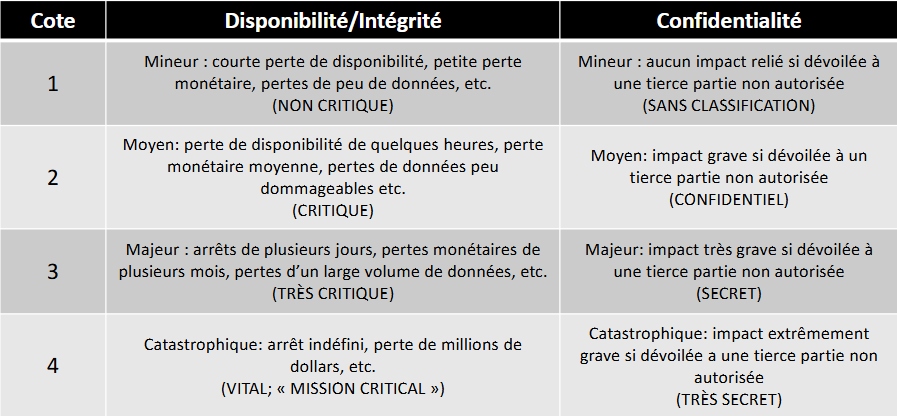
\includegraphics[width=1\linewidth]{static/échelle_risque.png}
\end{center}

\footnotesize \subsection{Analyse des risques}

\begin{center}
    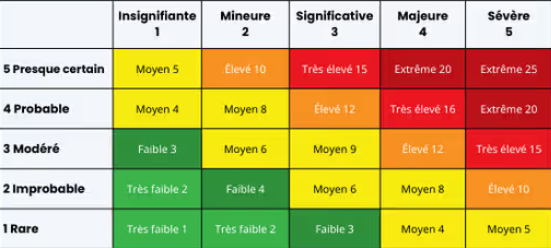
\includegraphics[width=1\linewidth]{static/matrice_risque.png}
\end{center}

% --- Cours 3 ---

\footnotesize \section{Modèle de Shannon}

\begin{center}
    \scriptsize source $\rightarrow$ codeur $\Rightarrow$ décodeur $\rightarrow$ récepteur
\end{center}

\begin{itemize}[leftmargin=0.5em,label=$\bullet$]
    \item \scriptsize \textbf{Alphabet}: $\Sigma = \{\sigma_{1}, \ldots, \sigma_{M}\}$
    \item \scriptsize \textbf{Taille} de $\Sigma = \lvert \Sigma \rvert = M$
\end{itemize}

\begin{flushleft}
    \scriptsize \textbf{Fonction de codage}
\end{flushleft}

\begin{itemize}[leftmargin=0.5em,label=$\bullet$]
    \item \scriptsize $F : \Sigma \rightarrow T$
    \begin{itemize}[leftmargin=0.5em,label={}]
        \item \scriptsize  $\tau = F(\sigma)$
    \end{itemize}
\end{itemize}

\begin{flushleft}
    \scriptsize \textbf{Fonction de décodage}
\end{flushleft}


\begin{itemize}[leftmargin=0.5em,label={}]
    \item \scriptsize $F^-1 : T \rightarrow \Sigma$
    \begin{itemize}[label={}]
        \item \scriptsize $\sigma^\prime = F^-1(\tau^\prime)$
    \end{itemize}
    \item \scriptsize \textbf{si} $\tau^\prime \neq \tau \rightarrow \sigma^\prime \neq \sigma$
    \begin{itemize}[label=$\bullet$]
        \item \scriptsize erreur dans le canal
    \end{itemize}
    \item \scriptsize \textbf{si} $\tau^\prime = \tau \rightarrow \sigma^\prime = \sigma$
    \begin{itemize}[label=$\bullet$]
        \item \scriptsize sans erreur
    \end{itemize}
\end{itemize}

\footnotesize \subsection{Correction d'erreur}

\begin{flushleft}
    \scriptsize source $\rightarrow$ codeur $\rightarrow$ ajout syndrome $\Rightarrow$ \text{corr.\ erreur} $\rightarrow$ décodeur $\rightarrow$ récepteur
\end{flushleft}

\footnotesize \subsection{Entropie de Shannon}

\begin{itemize}[leftmargin=0.0em,label={}]
    \item \scriptsize $H_{b}(X) = \sum_{i=1}^{n} \log_{b}(1/P_{i}) = -\sum_{i=1}^{n} P_{i} \log_{b}(P_{i})$
    \begin{itemize}[label=$\bullet$]
        \item \scriptsize bit/symbole b=2
    \end{itemize}
    \item \scriptsize Si alphabet équiprobable :
    \begin{itemize}[label={}]
        \item $H_{2}(X) = \log_{2}(\lvert \Sigma \rvert)$
    \end{itemize}
    \item \scriptsize Si non équiprobable (fréquence des symboles) :
    \begin{itemize}[label={}]
        \item \scriptsize $\hat{H} = -\sum_{i=1}^{n} f_{i} \log_{2}(f_{i})$
    \end{itemize}
    \item \scriptsize  Entropie en bloc (exemple \textbf{$S^{3}$}) :
    \begin{itemize}[label=$\bullet$]
        \item \scriptsize $P(A) = P(B) = \ldots = P(Z) = 1/26$
        \item \scriptsize Probabilité des séquences - toutes équiprobable
        \item \scriptsize (AAA, AAB, AAC, \ldots, ZZZ), nb de séquences $= N = 26^{3} = 17576$
        \item \scriptsize Probabilité d'une séquence $S_{i}^{3} = 1/N = 1/17576$
        \item Donc,
    \end{itemize}
    \item \scriptsize $H = \log_{2}(N) = \log_{2}(N) = \log_{2}(26^{3})$
    \begin{itemize}[label={}]
        \item \scriptsize $H = \log_{2}(\lvert \Sigma \rvert^{x})$
        \item \scriptsize $H = x \cdot \log_{2}(\lvert \Sigma \rvert)$
        \item \scriptsize $H = 3 \times  \log_{2}(26)$
    \end{itemize}
    \item \scriptsize  Entropie par bloc
    \begin{itemize}[label={}]
        \item \scriptsize $\frac{H(S^{b})/b}{\log_{2}(N)}$
    \end{itemize}
\end{itemize}

\footnotesize \subsection{Modèle de Shannon révisé}

\begin{flushleft}
    \scriptsize source $\xrightarrow{\sigma}$ $\underset{F}{\text{codeur}}$ $\xrightarrow{\tau}$ $\underset{E}{\text{chiffr.}}$ $\xRightarrow{\tau^{\prime}}$ $\underset{D}{\text{déchiff.}}$ $\xrightarrow{\tau}$ $\underset{F^{-1}}{\text{décodeur}}$ $\xrightarrow{\sigma}$ récepteur
\end{flushleft}

\footnotesize \section{Algorithmes classiques}

% --- Substitution ---

\footnotesize \subsection{Substitution}

\begin{itemize}[label=$\bullet$]
    \item \scriptsize chiffrement
    \begin{itemize}[label={}]
        \item \scriptsize $x \rightarrow \pi(x)$
    \end{itemize}
    \item \scriptsize clé
    \begin{itemize}[label={}]
        \item \scriptsize $\pi$: table de substitution
    \end{itemize}
\end{itemize}

% --- Transposition ---

\footnotesize \subsection{Transposition « bit shifting »}

\begin{center}
\begin{tabular}{|c|c|c|c|c|c|c|c|c|c|}
\hline
\scriptsize \textcircled{H} & e & l & l & o & w & o & r & l & d \\
\hline
\scriptsize 1 & 2 & 1 & 2 & 1 & 2 & 1 & 2 & 1 & 2 \\
\hline
\end{tabular}
\end{center}

\vspace{-0.5cm}

\begin{tabular}{ll}
\scriptsize \textbf{Rail 1 :} & \textcircled{H} \quad l \quad o \quad o \quad l \\
\scriptsize \textbf{Rail 2 :} & e \quad l \quad w \quad r \quad d \\
\end{tabular}

\vspace{0.1cm}
\scriptsize \textbf{Résultat :} \texttt{Hloolelwrd}

% --- César ---

\footnotesize \subsection{César}

\begin{itemize}[label=$\bullet$]
    \item \scriptsize chiffrement
    \begin{itemize}[label={}]
        \item \scriptsize $x \rightarrow x+3(\mod 26)$
    \end{itemize}
\end{itemize}

% ---  Décallage --

\footnotesize \subsection{Décallage}

\begin{itemize}[label=$\bullet$]
    \item \scriptsize chiffrement
    \begin{itemize}[label={}]
        \item \scriptsize $x \rightarrow x+k(\mod 26)$
    \end{itemize}
    \item \scriptsize clé
    \begin{itemize}[label={}]
        \item \scriptsize $k \in \{1 \ldots 26\}$
    \end{itemize}
\end{itemize}

% --- Afin ---

\footnotesize \subsection{Afin}

\begin{itemize}[label=$\bullet$]
    \item \scriptsize chiffrement
    \begin{itemize}[label={}]
        \item \scriptsize $x \rightarrow ax + b (\mod 26)$
    \end{itemize}
    \item \scriptsize clé
    \begin{itemize}[label={}]
        \item \scriptsize $(a,b) \in \{1 \ldots 26\}$
    \end{itemize}
\end{itemize}

% --- Algorithme de Vigenère ---

\footnotesize \subsection{Algorithme de Vigenère}

\begin{itemize}[label=$\bullet$]
    \item \scriptsize clé
    \begin{itemize}[label={}]
        \item \scriptsize $k = k_{1}, k_{2}, \ldots, k_{m}$
        \item \scriptsize mot / phrase de longueur m
    \end{itemize}
    \item \scriptsize chiffrement
    \begin{itemize}[label={}]
        \item \scriptsize $x_{i} \rightarrow (x_{i} + k_{i} \mod m) \mod 26$
    \end{itemize}
\end{itemize}

% -- Masque jetable ---

\footnotesize \subsection{Masque jetable}

\begin{itemize}[label=$\bullet$]
    \item \scriptsize $\Sigma = T = \{0, 1\}$
    \item \scriptsize Algorithme: XOR bit à bit du message et de la clé
\end{itemize}

% --- Cours 4 ---

% --- Cours 5 ---

% --- Cours 6 ---

% --- Cours 7 ---

% --- Cours 8 ---

% --- Cours 9 ---

% --- Cours 10 ---

% --- Cours 11 ---

% --- Cours 12 ---

\end{multicols}

\end{document}
